\documentclass{article}

\usepackage[utf8]{inputenc}
\usepackage{authblk}
\usepackage{hyperref}
\usepackage[margin=2cm]{geometry}
\usepackage{listings}
\usepackage{graphicx}
\lstset{
  language=bash,
  basicstyle=\ttfamily
}

\title{Espotifai\\
\vspace{10pt}
\large Automatic Playlist Recommender}
\author[]{Lucas Emanuel Resck Domingues}
\author[]{Lucas Machado Moschen}

\affil[]{\textit{School of Applied Mathematics}
\\ \textit{Getulio Vargas Foundation}}

\date{\today}

\begin{document}

\maketitle

\begin{center}
    \href{https://github.com/lucasresck/espotifai}{GitHub Repository}
\end{center}

\section{Project statement}

    \textbf{Question}: Which song should we recommend based on
    a playlist and user or context information?

    We can define playlist as a sequence of tracks (audio recordings).
    In this project we aim to study the playlist generation problem, that is,
    given a pool of tracks, a background knowledge about the user,
    and some metadata of songs and playlists, the goal is to create a sequence
    of tracks that satisfies some target as best as possible. The notebooks,
    scripts and work can be found in our repository.

\section{The Datasets}

In order to get user information, we generated a list of usernames in a
networked way.  We visited the Last.fm webpage of several artists and
considered three random users in the top listenings from three different
coutries: Brazil, USA and United Kingdom. Using only these usernames, through
the command \lstinline{generate_lastfm_users.py},  we get additional
Last.fm usernames using the \lstinline{user.getFriends} method from the API. 
With some loops, we can get the network (or part of it). It's possible to have
some bias, unknown yet.

Both databases were built using the Application Programming Interface (API) from the
website, in special
\href{https://developer.spotify.com/documentation/web-api/}{Spotify API} and
\href{https://www.last.fm/api/}{Last.fm API}. Both are great players in the
music business and that was the reason for us to use. 

\subsection{Spotify Database}

\subsection{Last.fm Database}

We used \href{https://github.com/pylast/pylast}{pyLast}
package for Python to help with the connection. It organizes all as an object
with several functions. However, in order to retrieve all the information, it
takes a long time to build all datasets: \textbf{Users info}, \textbf{Tracks
info}, \textbf{Artists info} and \textbf{Tags info}, because we retrive a lot
of information in different links from the same API. That's why in the first
analysis we only considered a subset. We got the users randomly from the whole
dataset of users. We saved the information in a \lstinline{json} format. The
variable types were fixed to help the analysis (convertion
\lstinline{string->integer}). The dates were converted to a standart type and
after to datetime. Actually, as we used an API, the data wasn't bad. We
created ids for tracks, tags and artists and save it in a \lstinline{.csv}
file. This structure allow us to save storage. 

The considered datasets were: 

\begin{enumerate}
  \item \textbf{Users}: information about if is subscriber, when he/she 
  has registered, playcounts, country, top artists and tracks and loved
  tracks. (no user had gender, age and number of playlists information and
  we deregarded.)
  \begin{itemize}
    \item Users: 1000; users with no information: 1.
    \item We are dealing with personal information generated by the user (like loved
    tracks) and by user's preferences (like top tracks)    
  \end{itemize}
  \item \textbf{Tracks}: information about reaching, playcounts, duration,
  listeners, similar tracks and top tags.
  \begin{itemize}
    \item tracks: 9902; tracks with no information: 311.
  \end{itemize} 
  \item \textbf{Artists}: information about number of listeners, plays, when
  he/she was published, top tracks, top tags and similar ones.
  \begin{itemize}
    \item artists: 1055; artists with no information: 0.
  \end{itemize}
  \item \textbf{Tags}: information about registration, taggings, reached
  people, top tracks and top artists.
  \begin{itemize}
    \item tags: 1843; tags with no information: 4
  \end{itemize} 
\end{enumerate}

\begin{figure}[!h]
  \centering
  \label{fig:top-loved}
  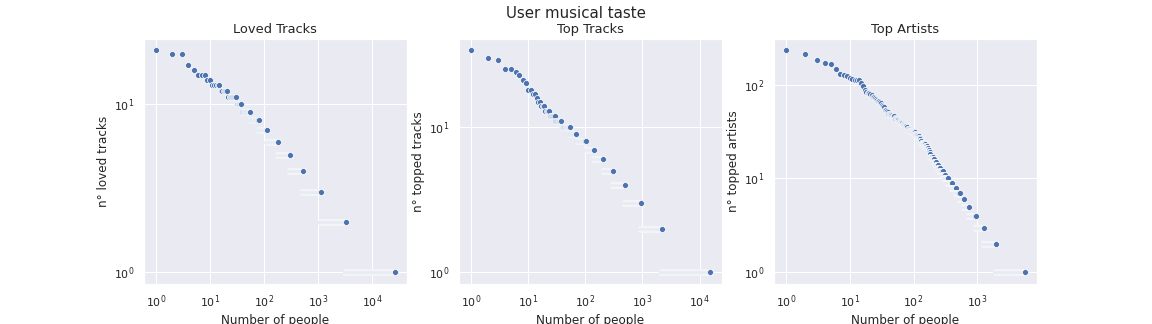
\includegraphics[width = \textwidth]{../../images/top-loved-tracks.png}
\end{figure}

\begin{figure}[!h]
  \centering
  \label{fig:artist-info}
  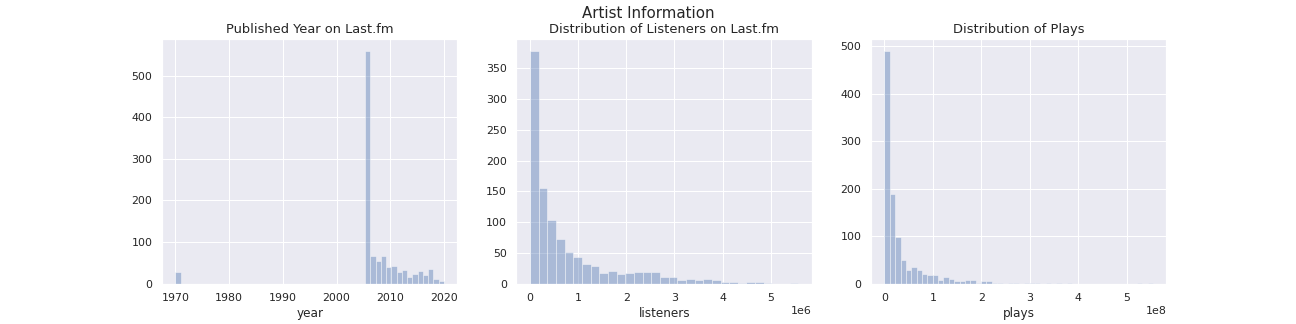
\includegraphics[width = \textwidth]{../../images/artist_info.png}
\end{figure}

\section{Gained Insights}

TO DO 

Ideas:
\begin{enumerate}
  \item Pareto's distribution in the data; 
  \item getSimilar is a good function from last.fm
  \item Last.fm has information about general aspects of the user, but it's
  not good to create models fow playlists. 
\end{enumerate}

\section{Baseline Model}

It's pretty simple and uses information retrieved from Last.fm. From a
playlist (from Spotify), we get all the artists who participate in at least
one song and attribute a weight of the number of times it appears in the playlist. After we get the 200 top artists of the user, weighted by the number of
times the user listened to him/her. With that information, we get the
intersection of the two. If it is empty, the method does not work, unhappily.
With the intersection, we take the 10 artists with major weight and for each,
we get the 10 top tracks and recommend the $n$ tracks with major weight
(number of playcounts by all the users in the plataform). 

\end{document}